\documentclass[a4paper,12pt,ngerman]{scrartcl}

% standard packages
\usepackage[german]{babel}
\usepackage[utf8x]{inputenc}
\usepackage[a4paper,margin=2.5cm]{geometry}

% additional packages
\usepackage[colorlinks=true,linkcolor=black,urlcolor=blue,
            citecolor=blue,anchorcolor=blue]{hyperref}
\usepackage{amsmath}
\usepackage{csquotes}
\usepackage{graphicx}
\usepackage{float}
\graphicspath{{bilder/}}

% dev chart 
\usepackage{tikz}
\usetikzlibrary{arrows.meta}
\usepackage{forest}
\forestset{qtree/.style={for tree={align=center, grow'=east, edge={green!50!black, -Latex}}}}

% specific packages which are less often needed
\usepackage[official]{eurosym}

% meta information
\title{DOSUAS - Die Symphonie des Sehens}
\subtitle{Jugend forscht 2018}
\author{Jonas Wanke und Yorick Zeschke}
\date{\today}

\begin{document}

\maketitle


\begin{abstract}
	DOSUAS (\textbf{D}evice for \textbf{O}rientation in \textbf{S}pace \textbf{U}sing 
	\textbf{A}udio \textbf{S}ignals) ist ein Gerät, welches es blinden Menschen ermöglicht,
	sich mithilfe von akustischen Signalen im Raum zu orientieren. Das wird erreicht, indem Bilder 
	einer 3D-Kamera mit verschiedenen Methoden algorithmisch in Töne umgerechnet werden,
	die Informationen über die aufgenommene Umgebung enthalten. Mit Übung kann der Träger des Gerätes 
	sich dann nach dem Hören dieser Töne im Raum orientieren und die Form, Entfernung und Ausrichtung 
	verschiedener Objekte bestimmen.
\end{abstract}

\tableofcontents

\newpage

\section{Einleitung}

Blinde Menschen hatten schon immer Probleme damit, sich im Raum zu orientieren.
Manche von ihnen, zum Beispiel \textit{Daniel Kish}, benutzen die Technik der 
\textit{menschlichen Echoortung}, ein Verfahren, bei dem
man regelmäßig mit dem Mund Klicklaute erzeugt und das Gehör darauf trainiert,
anhand der Reflexionen ein genaues Bild der Umgebung im Kopf zu erzeugen.
Forscher haben herausgefunden, dass sich dabei die Struktur des Gehirns verändert 
und Signale von den Ohren im Sehzentrum verarbeitet werden.
Mit genügend Übung schaffen es Blinde so zu \enquote{sehen} und können Fahrrad 
fahren oder in den Bergen klettern. \par 
Doch nicht jedem Blinden fällt es leicht und nicht jeder hat die Möglichkeit eine
solche Technik zu erlernen. Außerdem hat auch die menschliche Echoortung ihre
Grenzen und ist ab einem bestimmten Punkt nicht mehr erweiterbar, denn die Schallreflexionen
enthalten nur eine begrenzte Menge an Informationen, deren Potenzial irgendwann ausgeschöpft
ist. Hier kommt die 
Technologie ins Spiel. Von Tag zu Tag ergeben sich neue Möglichkeiten mithilfe 
der verschiedensten technischen Hilfsmittel Menschen das Leben zu erleichtern.
Geräte, wie 3D-Sensoren oder Kameras, können heutzutage schon oft sehr realistische
und detaillierte Bilder aufnehmen, die dem menschlichen Sehen nahe kommen. \par 
Relativ neu ist zum Beispiel die Technologie der \textit{Retina-Implantate}, die sich 
momentan aber noch im Anfangsstadium der Entwicklung befindet. Mit ihnen soll es in 
Zukunft möglich sein, dass Blinde wie nicht sehbehinderte Menschen sehen. Jedoch
können die Kosten von 75.000 \euro{} aufwärts selten von den Blinden selbst getragen
werden. Auch gibt es zu viele
blinde und sehbehinderte Menschen, als dass es möglich wäre, jeden mit einem so 
teuren Gerät zu versorgen.\par 
Verschiedene Firmen versuchen das Sehen technisch durch andere Sinne zu ersetzen.
Ein berühmtes Beispiel dafür ist der 
\enquote{BrainPort V100}\footnote{https://www.wicab.com/brainport-v100}, welcher 
Kamerasignale in elektronische Impulse umwandelt, die auf der Zunge spürbar
gemacht werden. Nachteile dieser
Technologie sind vor allem lange Lernprozesse, die nur mit ärztlicher Unterstützung
möglich sind, Probleme bei zu vielen Reizen oder große Ungenauigkeiten. Der Brainport V100 ermöglicht
zwar relativ genaues Erkennen von kleinen Objekten, wie Tassen oder Bücher, eignet sich aber weniger zum
Erkennen großer Räume und hilft daher der Orientierung nicht besonders.
Beispielsweise kann es passieren, dass ein Blinder beim Betrachten des Geschehens auf 
einer großen Straße nichts mehr wahrnimmt, weil der Tastsinn der Zunge
nicht für eine solche Reizüberlastung ausgelegt ist. Unsere Zunge ist zwar empfindlich, aber besitzt keine
\enquote{Auflösung}, die hoch genug ist, um größere Umgebungen auf einmal zu erkennen.\par 
Unser Gerät funktioniert gegensätzlich: Es ermöglicht 
Orientierung im Raum und eignet sich weniger gut für kleine Objekte. Aber mit dem Tastsinn können Menschen
sowieso Gegenstände viel genauer erfühlen, als man sie mit einem Sensor wie unserem sehen könnte.\par
Da unser Gehirn sehr anpassungsfähig ist und beeindruckende
Leistungen im Finden von Regelmäßigkeiten oder Mustern erbringt, ist der Ansatz,
andere Sinne zu verwenden, eine vielversprechende Strategie. Darauf setzt auch 
unser Projekt, DOSUAS, welches den Hörsinn verwenden möchte, um Blinden eine Hilfe
für Orientierung und Erkennung der Umwelt zu geben.

\newpage

\section{Funktionsweise}

Das Gerät besitzt momentan zwei Modi: den einfachen und den fortgeschrittenen Modus. Der einfache Modus
erlaubt eine grundlegende Orientierung und das Erkennen von großen Objekten, wobei Ergebnisse bereits
innerhalb der ersten Stunde des Trainings erkennbar waren (siehe Abschnitt \ref{testsAndResults}). Der
fortgeschrittene Modus ist für erfahrenere Personen geeignet und ermöglicht dem Nutzer, die Umrisse von
Gegenständen oder Strukturen fast jeder Art relativ genau zu erkennen. Allgemein gilt hierbei:
je mehr Details das Gerät darstellt und als Töne kodiert, desto länger dauert der Lernprozess. 
Daher unterscheiden wir auch zwischen beiden Modi. In Zukunft sind noch weitere geplant, aber mehr dazu im 
Ausblick.

\subsection{Verwendete Technologien}

Der wichtigste Teil dieses Projekts ist eine ToF-Kamera (\textit{Time of Flight}-Kamera), die neben herkömmlichen Farbfotos 
auch Tiefenbilder aufnehmen kann.
In diesen bekommt jeder Pixel einen Wert, der die Entfernung zur Kameralinse in mm angibt.
Der von uns verwendete \enquote{Cube Eye MDC500C}\footnote{http://www.cube-eye.co.kr/en/\#/spec/product_MDC500d.html}
Sensor hat eine Reichweite von $0,8 m$ bis $5,3 m$ und eine Auflösung von $320 \times 240$ Tiefenpixeln. 
ToF-Kameras messen die Entfernung mithilfe von Infrarotlicht (In unserem Fall beträgt die Wellenlänge $850nm$). Dieses geben sie mit mehreren (hier zwei) Dioden
ab und messen die reflektierten Strahlen mit einer Sensormatrix (auch Pixelarray) im Inneren der Kameralinse. 
Über die Zeit zwischen Aussenden und Empfangen kann die Entfernung präzise bestimmt werden.
Weil der Sensor seine eigene Lichtquelle besitzt, funktioniert er auch im Dunkeln und wird von Licht im 
sichtbaren Spektrum nur wenig gestört. Der Cube Eye MDC500C hat viele Vorteile, aber auch einige Nachteile, wie z.\,B. 
Probleme beim Erkennen von lichtdurchlässigen oder reflektierenden Objekten (z.\,B. Glasscheiben oder Spiegel). 
Auch ist die Mindestreichweite von ca. $80 cm$ in einigen Situationen unpraktisch. Für einen Prototypen sind das aber keine großen Probleme, da es uns momentan darum geht, die Funktionsweise der Idee zu demonstrieren und kein marktreifes
Gerät zu entwickeln. Wir haben diese Kamera ausgewählt, weil sie uns von einem 
Familienmitglied\footnote{Jan Nicklisch, Vater von Yorick Zeschke, arbeitet in der Firma
\enquote{DILAX}, welche ähnliche Sensoren für Personenzählsysteme verwendet} 
empfohlen wurde. Zudem besitzt der Sensor noch eine normale Kamera, die später genutzt werden soll, um Farben mit den 
3D-Daten zu kombinieren.
\begin{figure}[H]
	\centering
	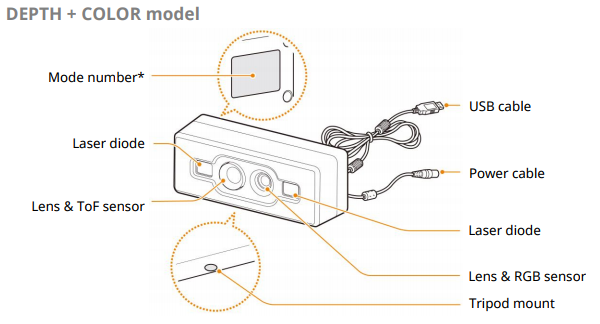
\includegraphics[width=0.6\textwidth]{cube_eye}
	\caption{beschriftetes Bild des Sensors aus dem Handbuch des Herstellers}
	\label{cube_eye_sensor}
\end{figure} \par
Einen weiteren wichtigen Teil des Projekts stellen Stereokopfhörer dar. Mit diesen kann der Eindruck
erzeugt werden, dass sich eine Tonquelle im dreidimensionalen
Raum befindet bzw. sich bewegt. Dieses Verfahren nutzen wir, um dem Träger des Geräts einen Eindruck
davon zu geben, in welcher Richtung sich ein Objekt befindet.\par 
Die dritte Komponente ist ein Laptop, der später durch einen kleineren Computer, wie z.B. ein \enquote{Raspberry Pi}
ersetzt werden soll. Dieser ist mit Kopfhörern und dem ToF-Sensor verbunden und führt unser Programm aus.\par 
Zusammen ergeben die drei Bestandteile (sowie ein externer Bleiakku für die ToF-Kamera) einen mobilen Prototypen, den wir am Ausstellungstag vorführen werden. Die Technik befindet sich dabei in einem Rucksack und der Sensor wird mit einem
umgebauten Stirnband am Kopf befestigt.
\begin{figure}[H]
	\centering
	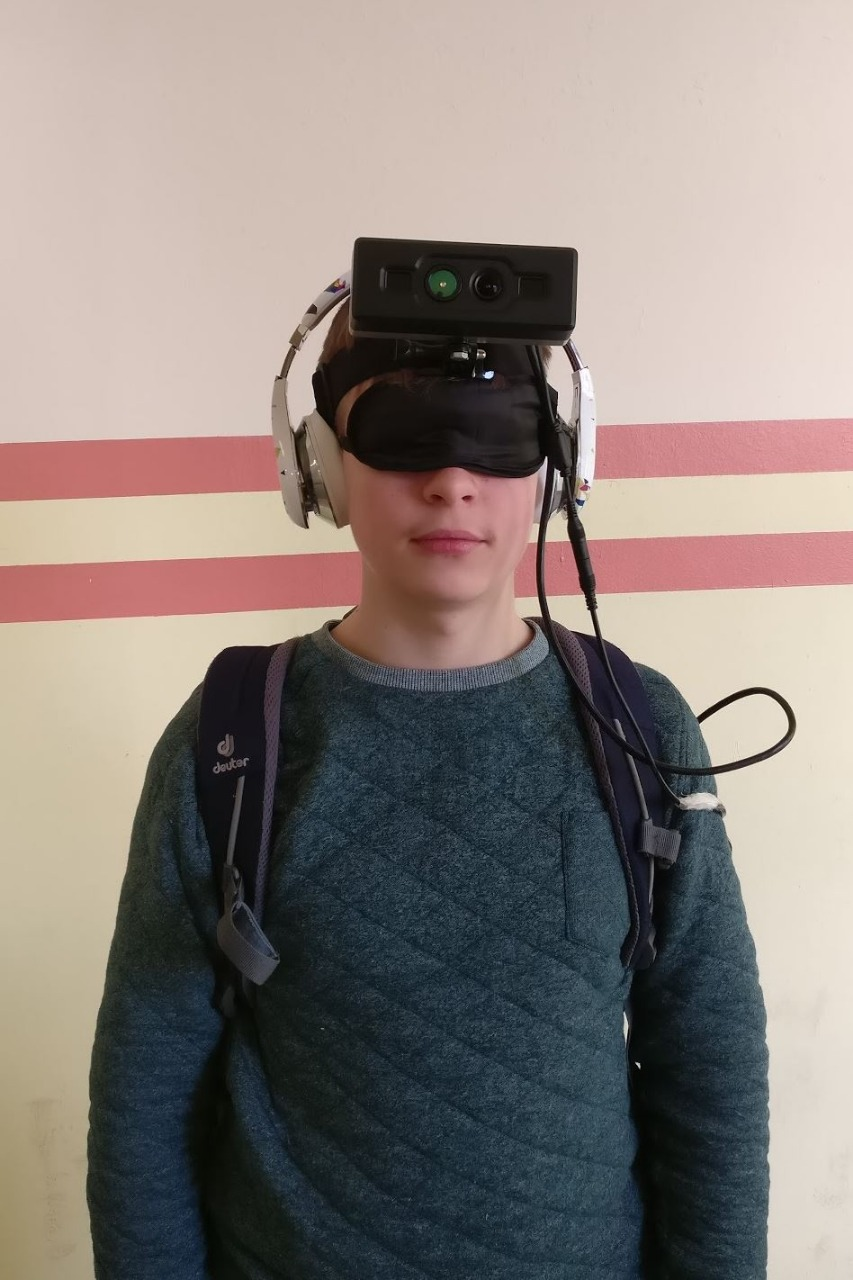
\includegraphics[width=0.4\textwidth]{device}
	\caption{Aufbau des portablen Prototyps}
	\label{dosuas_device}
\end{figure} 

\subsection{Softwarestruktur}

Das Programm ist in C++ geschrieben, da die API des ToF-Sensors dies erfordert und C++ eine objektorientierte und plattformunabhängige Sprache mit vielen Möglichkeiten ist. Momentan wird das Programm
auf Windows 10 (32 Bit) mit Visual Studio 2017 entwickelt. Wir verwenden folgende Libraries:
\begin{enumerate}
	\item \textit{MTF API} - Schnittstelle für die Steuerung des Cube Eye Sensors
	\item \textit{SFML} - einfache Multimedia-Bibliothek zum Abspielen von 3D-Sounds und Generieren von Tönen
\end{enumerate} 
Die Software selbst besteht im Moment aus 3 Modulen, die sich aber bis zur Ausstellung noch verändern 
können.
\begin{enumerate}
	\item \textit{sensorReader.cpp} - liest die Sensordaten aus und wandelt sie zur weiteren Verarbeitung in eine andere Struktur um
	\item \textit{imageProcessor.cpp} - beinhaltet Funktionen zum Filtern und Umwandeln der 3D-Bilder in Anweisungen zur akustischen Wiedergabe (Frequenzen und deren Spieldauer, Positionen der Tonquellen, Lautstärke etc.)
	\item \textit{audioPlayer.cpp} - generiert zu den Anweisungen passende Töne und spielt diese ab
\end{enumerate}
Den Quellcode finden Sie auf https://github.com/YpsilonZett/Dosuas.
Im folgenden sind nun der Ablauf des Programms sowie die Unterschiede der einzelnen Modi näher beschrieben.

\subsection{Vorverarbeitung}

Zuerst nimmt die Kamera ein Bild auf und stellt es als 2D-Matrix von $320 \times 240$ ($=76800$) natürlichen Zahlen dar.
In diesem Tiefenbild gibt jeder Pixel den Abstand zur nächsten lichtreflektierenden Region in $mm$ an. 
Dadurch erscheint eine gerade Fläche direkt vor dem Sensor jedoch auf dem Bild als nach außen gekrümmt, 
da das vom Sensor gesendete Infrarotlicht zu den Seiten der Fläche (und zurück) etwas länger
benötigt als zu deren Mitte. Aufgrund der kugelförmigen Ausbreitung der Lichtstrahlen von der Kameralinse ist das
Bild somit in einem Polarkoordinatensystem\footnote{jede Koordinate gibt eigentlich einen Winkel zwischen
	$0^{\circ}$ und $75^{\circ}$ (horizontal) bzw. $0^{\circ}$ und $60^{\circ}$ (vertikal) an,
weil der Sensor ein Sichtfeld von $75^{\circ} \times 60^{\circ}$ besitzt} dargestellt, welches nicht für unsere Weiterverarbeitung geeignet ist. Um das Problem der Verzerrung zu beheben und das Bild in ein kartesisches
Koordinatensystem umzurechnen, verwenden wir einen Undistortion\footnote{Dieser wurde vom Hersteller mitgeliefert und ist direkt in der Sensorkonfiguration einstellbar}-Algorithmus.
Die Abbildung zeigt ein verzerrtes Bild (Darstellung als Punktwolke\footnote{ggf. geordnete Menge von Punkten im karthesischen Koordinatensystem}), vor der Anwendung des Undistortion-Algorithmus.
\begin{figure}[H] \label{distorted_pointcloud_img}
	\centering
	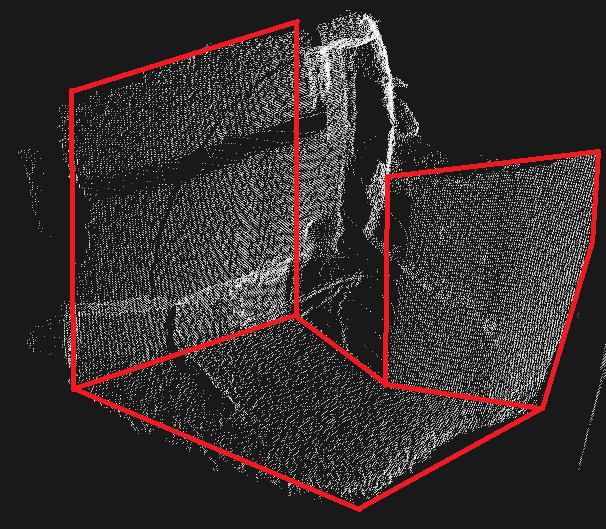
\includegraphics[width=0.6\textwidth]{no_undistortion2}
	\caption{verzerrte Punktwolke mit Messfehlern}
\end{figure}
Wie in Abb. \ref{distorted_pointcloud_img} zu sehen ist, wirkt eine ebene Fläche wie ein Teil einer Kugeloberfläche. Mit Rot sind hier die ungefähren Flächen ohne Verzerrung markiert, damit die Abweichung vom Original erkennbar ist.
Dieser Raum enthält viele Flächen und ist relativ einfach aufgebaut, weshalb er sich als einfache Testumgebung eignet.
\begin{figure}[H]
	\centering
	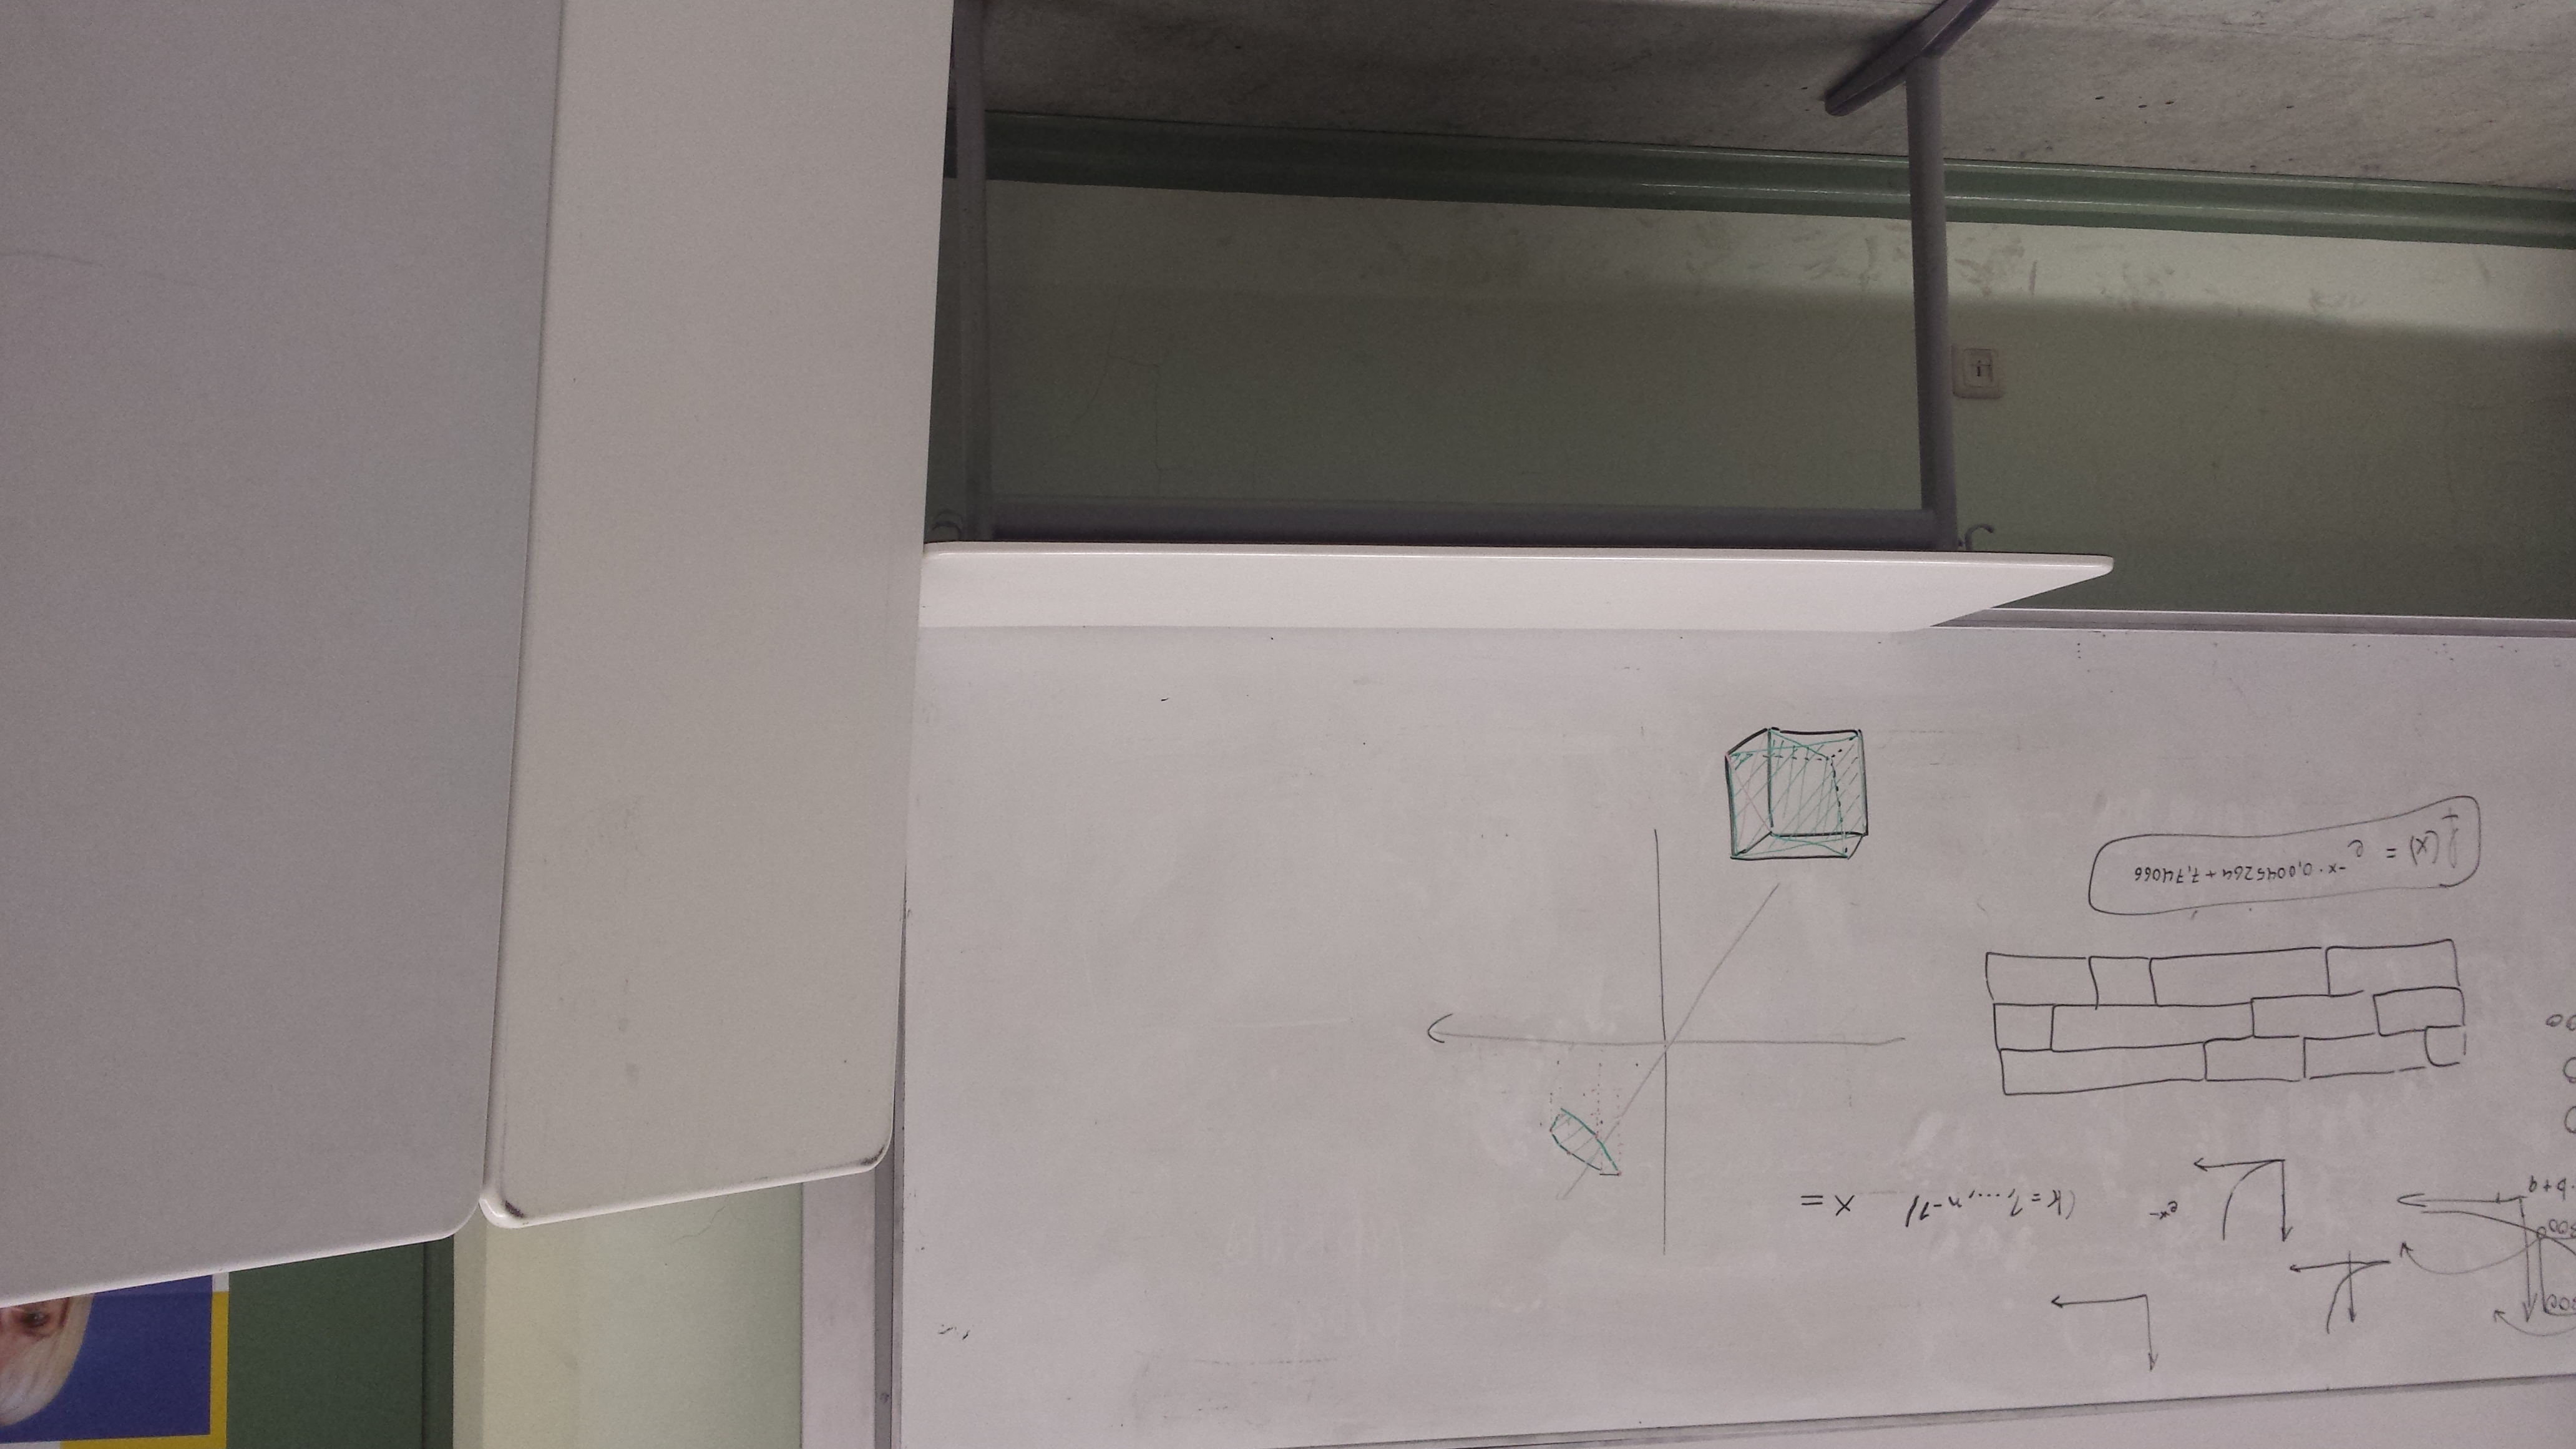
\includegraphics[angle=180,width=0.6\textwidth]{20180125_171703}
	\caption{Kamerabild des Raumes aus Abb. \ref{room_at_school}}
	\label{room_at_school}
\end{figure} \par
Die nächste Abbildung (Abb. \ref{before_filtering}) zeigt
die Aufnahme des selben Zimmers, in der die Wände gerade erscheinen. Durch die Visualisierung entsteht
der Eindruck, dass die Flächen Streifen (sogenannte Moir\'{e} Muster) enthalten. Das liegt jedoch an der
Visualisierung und hat nichts mit dem eigentlichen Bild zu tun. Die dünnen Linien rechts im Bild sind Punkte
mit der z-Koordinate 0, was Messfehler anzeigt. Diese entstehen, wenn etwas zu nah, zu weit oder zu stark
reflektierend ist, um von Sensor erkannt zu werden. Diese werden im weiteren Verlauf entfernt.
\begin{figure}[H]
	\centering
	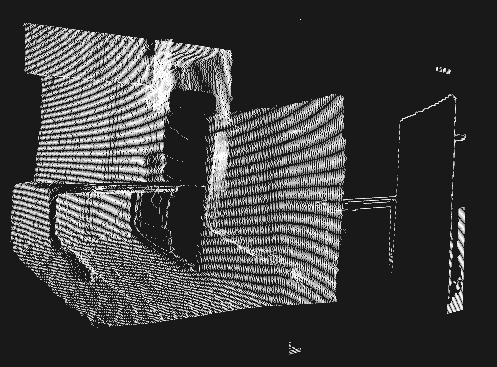
\includegraphics[width=0.6\textwidth]{before_filtering}
	\caption{algorithmisch korrigierte Punktwolke ohne Verzerrung}
	\label{before_filtering}
\end{figure} 

\subsection{Einfacher Modus}

Der einfache Modus stellt eine Art horizontalen Schnitt durch das Bild als Ton dar. Dieser enthält Informationen
über die Position auf der x-Achse (links, rechts und Werte dazwischen) sowie Entfernung einer Region, welche der Nutzer verwenden kann,
um sich grob zu orientieren. Die x-Position wird mithilfe von Stereosound dargestellt. Mit einfachen Kopfhörern und etwas Übung
kann man sehr genau bestimmen, in welche Richtung und wie weit entfernt sich eine Tonquelle befindet. Die Entfernung wird
durch die Tonhöhe angegeben, wobei etwas nahes als hoher Ton und etwas weiter entferntes als tiefer Ton gehört wird.
Nach einigem Experimentieren stellte sich heraus, dass Töne zwischen $300 Hz$ und $2300 Hz$ als angenehm empfunden werden und sich
auch längere Zeit (bei angemessener Lautstärke) ertragen lassen. \par 
Die Kombination aus Position und Frequenz ermöglicht es, im
einfachen Modus einen \enquote{Querschnitt} durch das Bild darzustellen. Es ist jedoch nicht besonders hilfreich, 
den Querschnitt an einer festgelegten Höhe durchzuführen. Wenn man z.\,B. im Raum aus Abb. \ref{room_at_school} den Schnitt im oberen Viertel des Bildes durchführen würde, würde er keine Informationen über den Tisch, der dichter als
die Wand liegt, enthalten. Daher teilen wir das Bild in Spalten, nehmen aus jeder Spalte den \enquote{nächsten} Voxel 
(mit der kleinsten z-Koordinate), generieren einen Ton für ihn und setzten diese Töne zu einem Tonverlauf zusammen. \par
Bei so einem Tonverlauf entsteht der Eindruck, dass die Tonquelle gleichmäßig von links nach rechts wandert und dabei ständig
die Tonhöhe ändert. Wir nennen so einen Tonverlauf \enquote{Radar Swipe}, da er einem Radarscan ähnelt.
Um Wände, Türen, Menschen und große Gegenstände (z.\,B. Schränke oder Tische) zu erkennen reichen diese Informationen völlig aus. So kann man also in den meisten Räumen umherlaufen und sich relativ frei bewegen.\par
Zum Beispiel könnte ein Ton, der in der linken Bildhälfte hoch anfängt, dann langsam tiefer wird und 
in der rechten Bildhälfte gleich bleibt, eine schräge Wand darstellen, die in einiger Entfernung in eine
zum Nutzer parallele Wand übergeht. Ein solch einfaches Beispiel kommt in der Realität zwar selten vor, und meistens gibt es
noch eine Menge Störgeräusche, aber näheres dazu im Abschnitt \ref{testsAndResults}.\par 
Momentan beträgt die Dauer zum Abspielen eines Bildes fünf Sekunden, gefolgt von einer halbsekündigen Pause.
Diese Dauer kann noch verkürzt werden, jedoch erfordert dies ein gewisses 
Training, weil der Mensch üben muss, mehr Informationen in kürzerer Zeit zu verarbeiten. Zusammen mit 
einer Verkürzung der Pausen zwischen Aufnahmen hoffen wir die Zeit für einen Programmzyklus auf ungefähr
zweieinhalb bis vier Sekunden zu reduzieren.

\subsection{Fortgeschrittener Modus}

In diesem Modus wird das gesamte Bild, also ein dreidimensionales Modell der Umgebung, als Töne dargestellt. 
Der Nutzer soll ein genaues Gefühl dafür bekommen, welche Umrisse einzelne Gegenstände haben und so die Form, Entfernung und Ausrichtung aller mittelgroßen und großen Objekte in einem Raum bestimmen können. \par 
Wir Menschen können an einem Ton im Wesentlichen drei
Eigenschaften ausmachen: Lautstärke, Position und Höhe. Wir reden hier von reinen Sinuswellen, da diese momentan für 
das Projekt ausreichen. Später kann man noch komplexere Töne einbauen, aber das würde das Lernen erschweren
und ist momentan nicht nötig. Die drei genannten Eigenschaften sollten, wenn mit dem Gehör viele Informationen
verarbeitet werden sollen, alle genutzt werden. Es ist wichtig anzumerken, dass Tonhöhe und Lautstärke viel genauer
wahrgenommen werden können als die Position, und wir diese daher überwiegend verwenden. \par 
Die Stereosound-Position übernimmt hier wieder die Funktion der x-Achse im Bild. Wie beim vorherigen Radar Swipe bewegt
sich eine Tonquelle gleichmäßig vom linken bis zum rechten Rand des Sichtfeldes. Wieder wird das Bild in Spalten 
unterteilt, diesmal jedoch in sehr viel geringer aufgelöste. Eine Spalte besteht nur aus 24 Voxeln.
Jedem dieser Voxel wird nun eine Frequenz zugeordnet, die der Höhe im Bild (y-Koordinate) entspricht.
Voxel am unteren Bildrand bekommen eine Frequenz von 220 Hz und Voxel am oberen Rand eine von 880 Hz. Die 24 
Pixel-Frequenzen bilden genau zwei Oktaven, wobei die Frequenzen danach ausgesucht wurden, einen harmonischen Klang zu erzeugen.
Jedem der Pixel wird nun eine Lautstärke zugeordnet, die die Entfernung (z-Koordinate) wiedergibt. Eine geringere
z-Koordinate entspricht einem lauteren Ton. Dies erscheint intuitiv, da nähere Objekte meist lautere Töne abgeben.\par 
Beim Abspielen des Tones erklingen alle Pixel einer Spalte gleichzeitig und bilden so einen Akkord aus 24 Tönen 
mit unterschiedlichen Lautstärken. Alle diese Akkorde (es gibt 32 Spalten) werden hintereinander abgespielt, während
sich die Tonquelle entsprechend der x-Koordinate einer Spalte bewegt. Zusammen bilden sie eine komplexe Melodie.
Zusammengefasst: x-Koordinate $\hat{=}$ Stereosound-Position, y-Koordinate $\hat{=}$ Frequenz und z-Koordinate $\hat{=}$ Lautstärke.

\subsubsection{Warum ist dies sinnvoll?}

Wir denken, dass dieses Verfahren eine geeignete Modellierung von 3D-Daten durch Töne ist. Wir wollen hier einige 
Fragen beantworten, die man sich unserer Wahl betreffend stellen könnte und unsere Entscheidungen begründen.
\begin{enumerate}
	\item \textbf{Warum benutzen wir keine Kopfhörer mit 3D-Audio?} - \textit{Man könnte die
	räumliche Position der 3D-Audio Tonquelle benutzen, um genauere Informationen über die Position eines
	Objektes anzuzeigen. Bei unseren Versuchen ist uns aber aufgefallen, dass es sehr schwer ist, die y-Koordinate einer
	3D-Audioquelle auch nur annähernd genau zu bestimmen. Um eine auf der z-Achse verschobene Tonquelle 
	darzustellen benötigt man die Lautstärke, die wir aber bereits verwenden. Deshalb	bleiben wir beim einfachen Stereo.}
	\item \textbf{Warum werden Frequenzen für die Höhe im Bild und nicht für die Entfernung verwendet?} - \textit{Würden wir Frequenzen für die Entfernung verwenden, müssten wir die Lautstärke verwenden, um Höhe auf dem Bild darzustellen. Dann wären aber nur die oberen Reihen des Bildes 
	hörbar, da das Gehör sich bei vielen Tönen auf die lautesten konzentriert. Diese Eigenschaft nutzen wir bei 
	unserer Version viel besser aus, 
	um das Gehirn dazu zu bringen, nähere Regionen genauer zu erkennen, da diese wichtiger sind.}
	\item \textbf{Wie kann das Gehör mit den vielen verschiedenen Frequenzen umgehen?} - \textit{Wie bereits gesagt, filtert das 
	Gehör bei vielen Tönen diejenigen heraus, die uns am wichtigsten erscheinen. Man bezeichnet dieses Phänomen als Cocktailparty-Effekt 
	oder selektives Hören. Wenn wir uns auf bestimmte Töne konzentrieren (z.B. die Stimme einer Person bei einer Unterhaltung vieler
	Personen) nehmen wir diese bis zu dreimal lauter wahr, als sie eigentlich sind. Bei den von uns erzeugten Akkorden stechen meistens
	zusammengesetzte oder einzelne Töne, die lauter als der Rest sind, heraus. Dadurch konzentrieren wir uns auf diese und nehmen sie noch deutlicher wahr. Mit etwas Übung kann man auch aus einem Akkord von vielen Tönen 
	die einzelnen heraushören und die Höhe so noch deutlicher wahrnehmen.}
\end{enumerate}

\newpage

\section{Praxistests} \label{testsAndResults}

Wir haben DOSUAS in verschiedenen Umgebungen getestet und werden Ihnen am Ausstellungstag einen Prototypen vorführen.

\subsection{Einfacher Modus}

Es stellte sich heraus, dass zum Üben der Handhabung des Gerätes mittelgroße Räume mit einfachen
Formen am geeignetsten sind. Die Räume dürfen aber nicht zu groß sein, da der Sensor eine maximale Reichweite
von $5,3 m$ besitzt. Auch in zu kleinen Räumen eignet sich das Gerät nicht, denn der Sensor hat eine Mindestreichweite von $0,8 m$.
Am Anfang sind Räume ohne viele kleine Objekte und mit großen Flächen wie Wänden einfacher, da die erzeugten Töne gleichmäßiger sind.
Hier sieht man einen anderen Raum, an dessen Beispiel die Töne beschreiben werden, die von unserem Gerät erzeugt werden.
\begin{figure}[H]
	\centering
	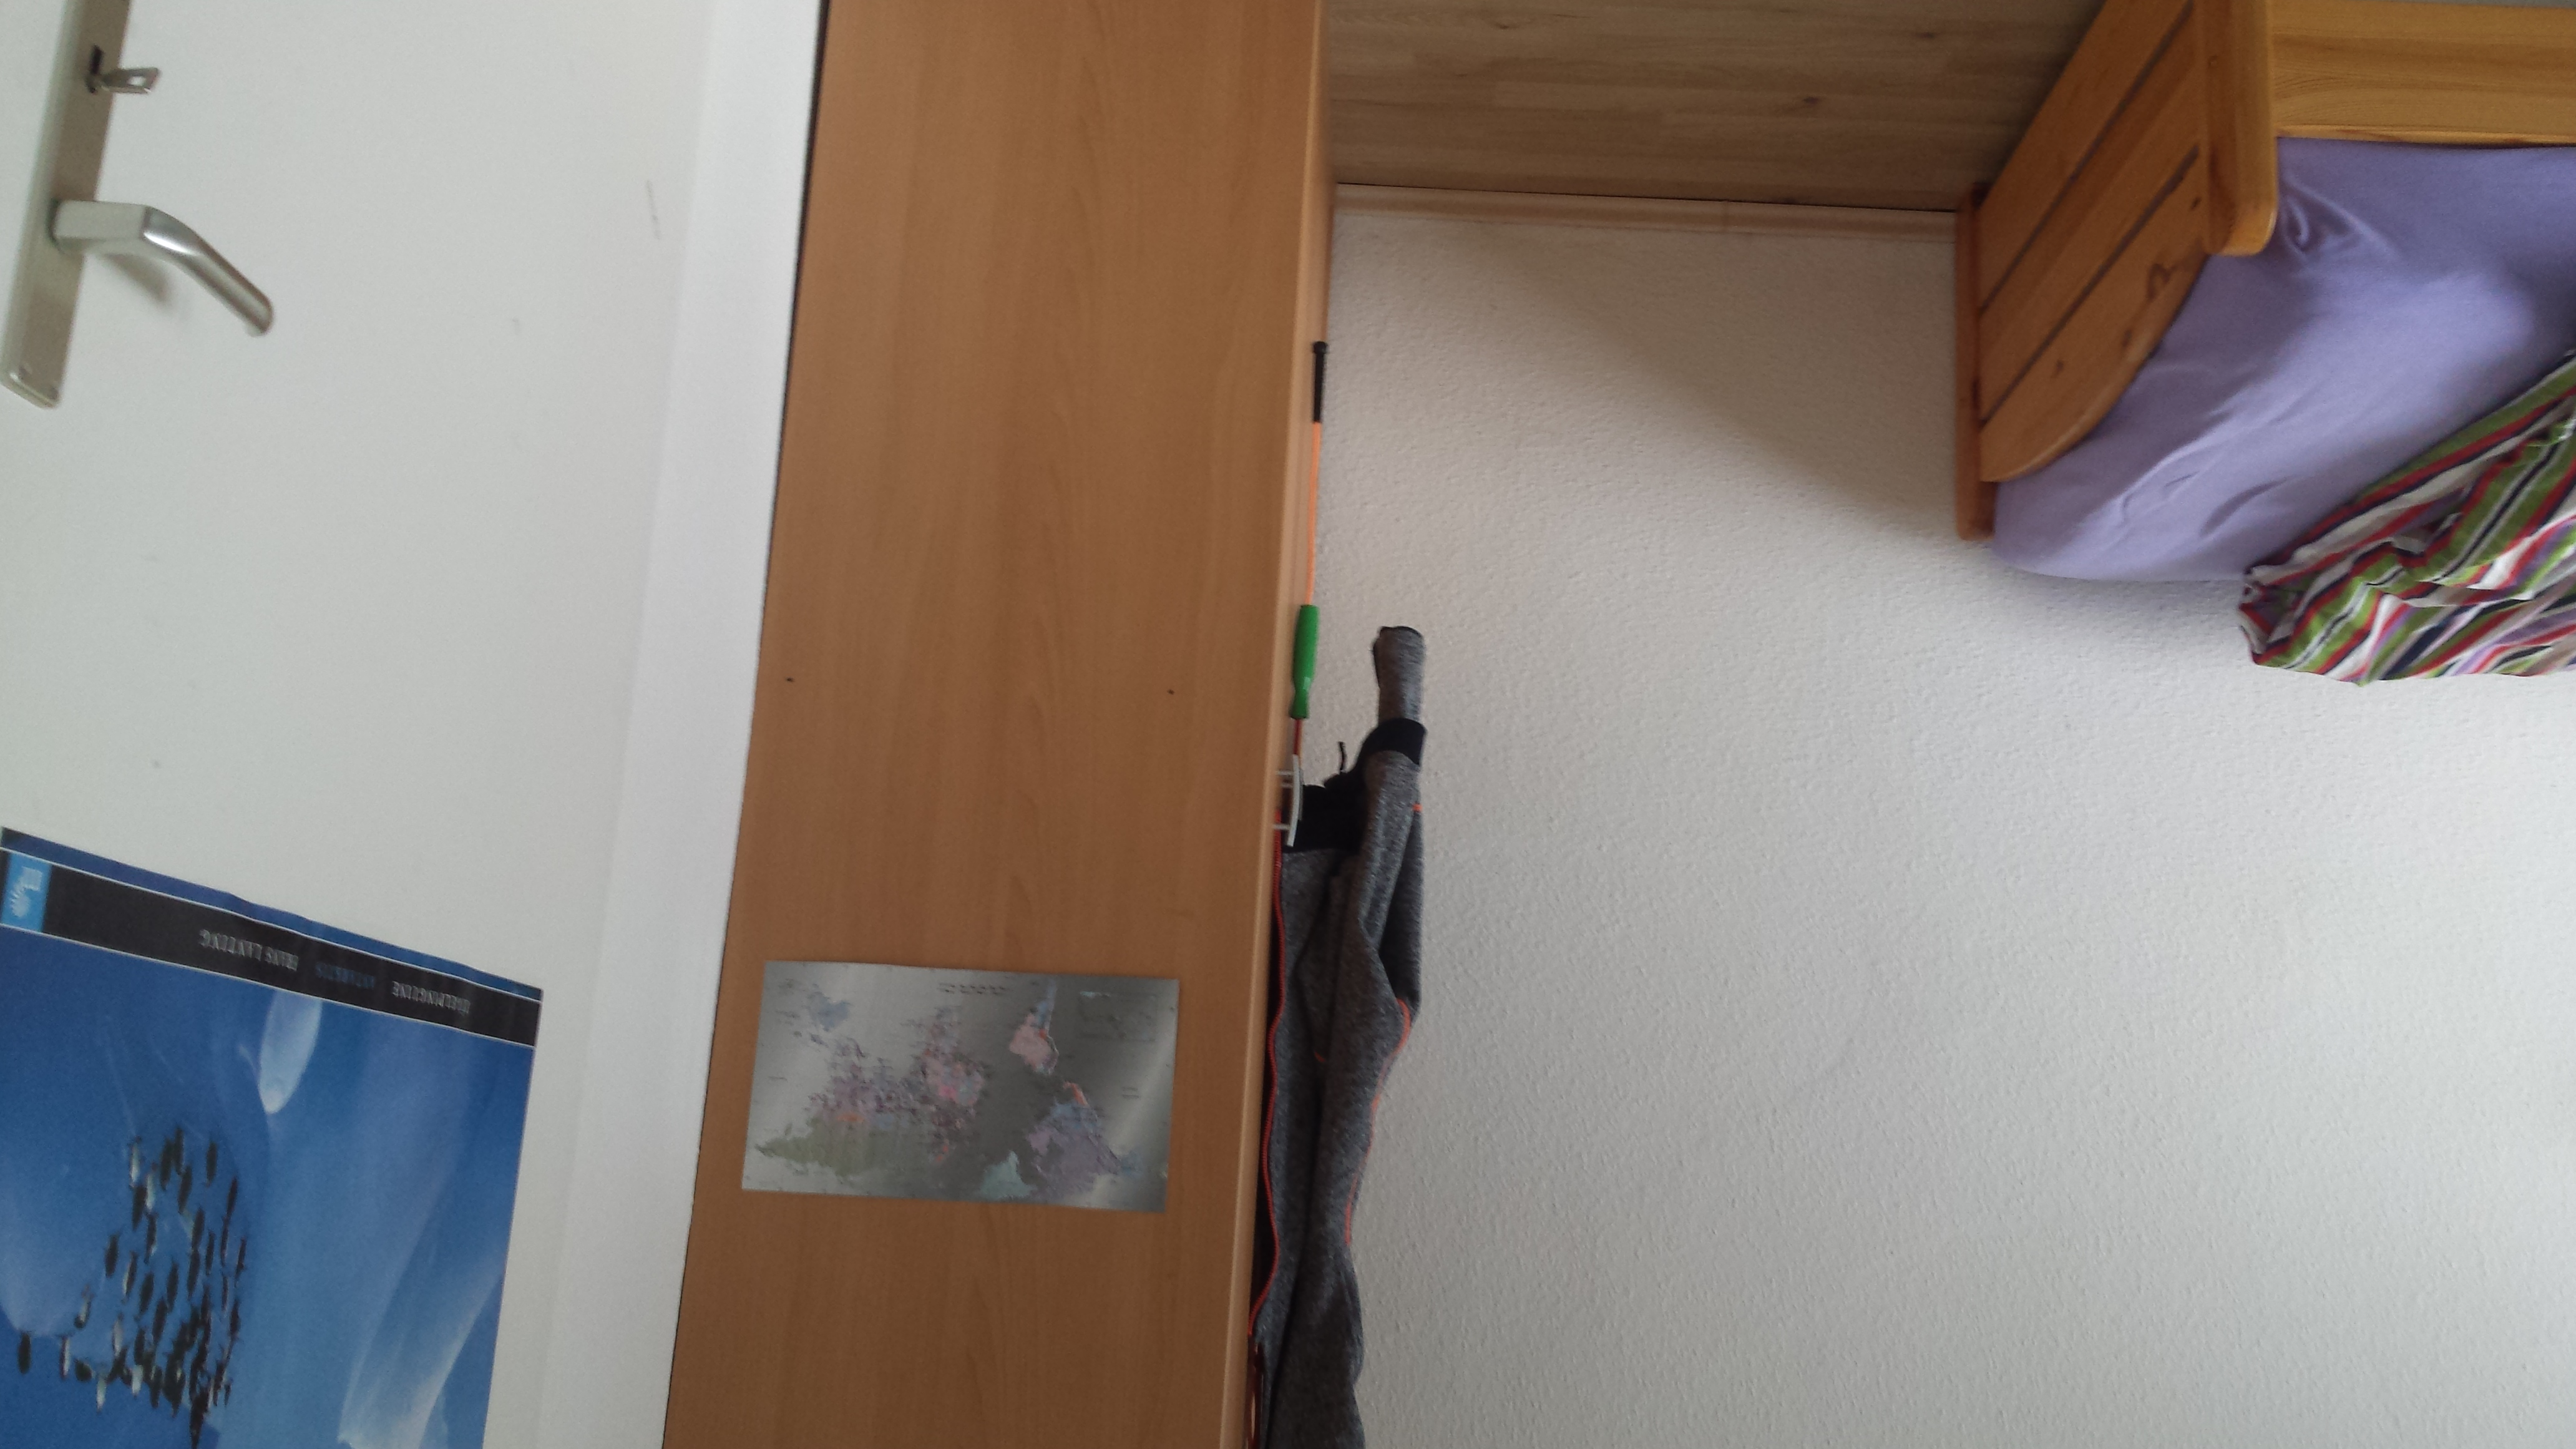
\includegraphics[angle=180,width=0.7\textwidth]{20180120_114953}
	\caption{Kamerabild eines anderen Raumes}
	\label{normal_picture}
\end{figure} \par
Man hört beim Betrachten dieses Raumes einen Ton, der etwa eine halbe Sekunde seine Frequenz (von ca. $550 Hz$) nicht verändert und sich anhört, als würde er von links kommen. Dieser Ton wird durch das Bett
erzeugt. Als nächstes wird der Ton über etwa eine halbe Sekunde gleichmäßig tiefer (bis $340 Hz$); 
jetzt ist unsere virtuelle Tonquelle an der Wand des Raumes angekommen. Der Ton steigt nun über $1\frac{1}{2}$ Sekunden sehr langsam an (auf ca. $360 Hz$), denn die Wand hat eine leichte Neigung. 
Danach hört man eine Art Sprung, bei dem der Ton ruckartig von $360 Hz$ zurück auf $550 Hz$ wechselt. An solchen Auffälligkeiten kann man Kanten, Öffnungen oder spitze Gegenstände erkennen, was für Blinde sehr wichtig
ist. Dieser Ton repräsentiert den Übergang von der Wand zum Schrank, der weiter vorne steht. Außerdem hört
man die virtuelle Tonquelle in diesem Moment direkt in der Mitte des Hörfeldes, was dem Nutzer anzeigt, dass sich
die Kante fast genau vor ihm befindet. Über ungefähr eine Sekunde bleibt die Tonhöhe wieder gleich, nur die Position
verändert sich; man hört die Fläche des Schranks. Über die restlichen $1\frac{1}{2}$ Sekunden steigt der Ton mit 
gleichbleibender Geschwindigkeit an und die Tonquelle wandert nach rechts.
Hier hört man die Tür und am Ende eine kurze \enquote{Spitze}, die die Türklinke darstellt. Am Ende hat der Ton
eine Frequenz von ca. $790 Hz$.\par 
Wir hoffen, dass Sie sich nun ein Bild davon machen können, wie sich die Welt mit DOSUAS anhört. Nach einem
halbstündigen Training mit dem Gerät waren unsere Testpersonen\footnote{Yorick Zeschke, Jonas Wanke, Petra Zeschke und Peter Kreißig} in der Lage (natürlich mit verbundenen Augen) in Schulräumen und Gängen
Wände und Türen zu erkennen, deren Ausrichtung und Entfernung sie beschreiben konnten, ohne sie gesehen zu haben.
Außerdem konnten sie sagen, ob eine Tür offen, halboffen oder geschlossen ist. Nach einer weiteren halben Stunde
war es ihnen möglich Menschen, Tische, Schränke und deren ungefähre Ausrichtung zu bestimmen. \par
Wir haben bereits einige wiederkehrende Muster gefunden, die auf bestimmte Objekte in einem Raum hindeuten:
\begin{figure}[h]
	\begin{tabular}{| p{0.4\textwidth} | p{0.5\textwidth} |}
		\hline
		\textbf{Objekt} & \textbf{Beschreibung des Tons} \\ \hline
		Wand oder große Fläche & gleichmäßige und ununterbrochene Änderung der Tonhöhe \\ \hline
		Kante, Ecke, sehr steile Fläche oder spitzer Gegenstand & \enquote{Sprung} von einer Tonhöhe zu einer 
		anderen \\ \hline
		Tür, Öffnung oder Loch (über die gesamte Höhe) & gleichmäßiger Ton (z.B. Wand), dann Sprung (Kante), wieder gleichmäßiger Ton
		(z.B. Gang hinter der Tür), noch ein Sprung und dann wieder ein gleichmäßiger Ton (Wand geht weiter) \\ \hline 
		Mensch oder Säule & gleichmäßiger Ton (z.B. Wand), dann \enquote{kreisförmiger}\footnotemark \,Ton, dann wieder ein gleichmäßiger Ton \\ \hline
		unregelmäßiges Objekt (z.B. Garderobe mit Kleidung oder Computer auf einem Tisch) & zitternd\footnotemark erscheinender Ton \\ \hline 
	\end{tabular}
\end{figure} \par
\footnotetext{Intuitiv würde man so einen Ton wohl
	als kreisförmig beschreiben. Der Frequenzverlauf kann durch eine nach unten geöffnete, gestauchte Parabel angenähert werden.}
\footnotetext{weil der Ton schnell zwischen verschiedenen Frequenzen wechselt} 
Wir wollen das Gerät noch mit
weiteren Leuten testen und sehen, wie schnell der Umgang damit erlernt werden kann. Wir vermuten, dass man nach einigen 
Tagen Selbsttraining im Stande ist, ohne Hilfe durch noch nie gesehene Räume zu gehen, ohne dabei irgendwo anzustoßen und
den Weg nach draußen wiederzufinden. Längeres Üben oder technische Verbesserungen bieten ungeahnte
Möglichkeiten. Doch das Gerät ist und bleibt zurzeit nur ein Prototyp. 

\subsection{Fortgeschrittener Modus}

Wir sind im Moment dabei, den fortgeschrittenen Modus mit verschiedenen Leute zu testen und die Orientierung damit zu üben. Bisher
ist es einzelnen Personen gelungen, mit diesem Modus ein Orientierungsvermögen zu erreichen, welches wesentlich besser ist als
beim einfachen Modus. Es hat sich auch mit Sicherheit gezeigt, das die Höhe von Objekten oder deren Position auf der
y-Achse bestimmbar ist, was den wesentlichen Vorteil gegenüber dem einfachen Modus darstellt. Zudem stellte sich heraus, dass die Lernkurve mit
dem fortgeschrittenen Modus etwas flacher ist und bis zu 10 Stunden benötigt werden, um sich damit gut zu orientieren.
Bis zum Wettbewerb werden wir aber noch weiter üben und den fortgeschrittenen Modus anpassen, weiterentwickeln und
umfassender testen. Die Testergebnisse werden wir Ihnen dann präsentieren.

\newpage

\section{Diskussion}

Im folgenden wollen wir kurz diskutieren, was wir für das Projekt planen und inwiefern man das
Gerät nutzen und weiterentwickeln kann und sollte. Außerdem fassen wir die durch die Entwicklung und Forschung am Projekt DOSUAS gewonnenen Erkenntnisse im Fazit zusammen.

\subsection{Entwicklung}

Hier sehen Sie eine Zusammenfassung der Entwicklung des Projekts. Hoffentlich können Sie nun verstehen, welche Ideen und Lösungsansätze 
wir verfolgt haben und warum wir uns in bestimmten Situationen für einen Entwicklungsweg entschieden haben.\par
\begin{forest}
	qtree
	[{Start}, name=start, s sep=0.5cm
	[{automatisierte Echoortung\\ via Ultraschall}
	[{aufwändige Entwicklung,\\ schlechtere Qualität als\\ menschliche Echoortung,\\ langer Lernprozess}, name=us_end, edge={red}]]
	[{Modellierung großer\\ Objekte als Tonquellen}
	[{zu wenig Informationen,\\ schlechte Orientierung}, name=objects_end, edge={red}]]
	[, no edge]
	[, no edge]
	[, no edge]
	[{2D Radar-Swipe\\ (jetziger Anfänger-\\Modus)}
	[{Verbesserter Anfänger-Modus\\ (beim Regionalwettbewerb vorgestellt)}]
	[{Fortgeschrittenen-\\Modus}
	[{siehe Ausblick}]]]]
	\useasboundingbox ([xshift=1cm, yshift=2.5cm]current bounding box.north west) rectangle (current bounding box.south east);
	\draw [green!50!black, -Latex] (us_end.north west) to [out=160, in=60] node[midway, above, black] {Abbruch nach Regionalwettbewerb} (0.2cm, 3.5cm) to [out=240, in=100] (start.north);
	\draw [green!50!black, -Latex] (objects_end.south west) to [bend left=20] node[midway, below, xshift=1.5cm, black] {Abbruch nach Regionalwettbewerb} (start.south east);
\end{forest}
%\begin{figure}[H]
%	\centering
%	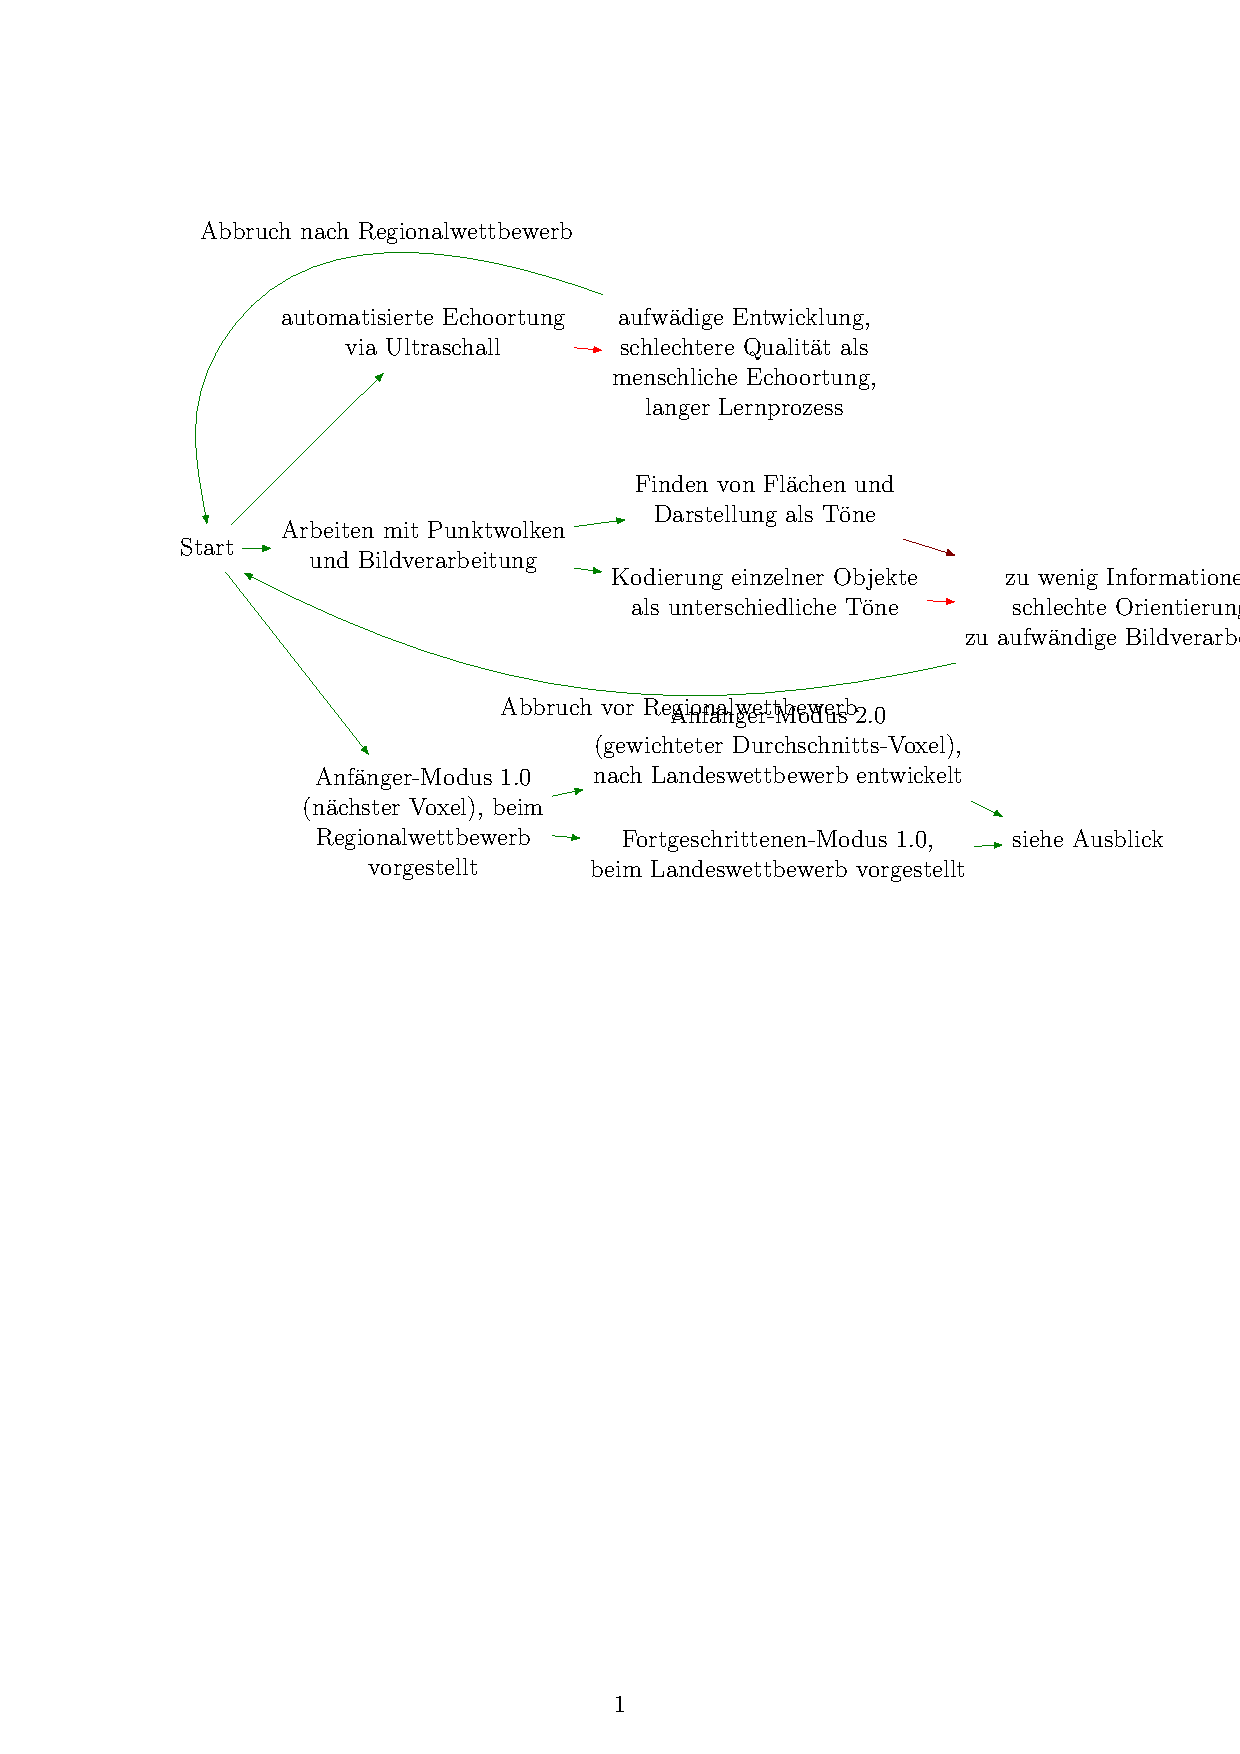
\includegraphics[width=0.85\textwidth]{dev_chart}
%	\label{dev_chart}
%\end{figure} 

\subsection{Ausblick}

Es gibt noch sehr viele Möglichkeiten, um das Projekt weiterzuentwickeln. Einige vielversprechende
möchten wir hier auflisten. Die Entwicklungen sind nach ihrer Komplexität und Wichtigkeit geordnet.
In Entwicklung (vermutlich bis zum Wettbewerb fertig):
\begin{enumerate}
	\item Verbesserung der Genauigkeit, z.B durch ein größeres Frequenzspektrum oder größere Intervalle (z.B. Quinten) in den
	 Akkorden beim fortgeschrittenen Modus
	\item Verkürzung der Abspieldauer, um das Sehen zu beschleunigen
	\item Entwickelung und Testen eines neues Modus, der Bilder durch Kanten von Objekten beschreibt (\enquote{zeichnet}) 
	\item Verbesserung der Portabilität durch Verkleinerung des Geräts, z.B. Laptop durch Raspberry Pi ersetzen oder das Programm per
	Handy-App steuern
	\item Einbauen von Texterkennung, sodass DOSUAS Texte vorlesen kann, die nicht in Braille geschrieben sind
\end{enumerate}
Ideen:
\begin{enumerate} 
	\item Entwickelung eines Echtzeit-Modus, um die Wahrnehmung zu beschleunigen
	\item Einbauen von Gesichts- und Objekterkennung, z.B. mit Machine Learning, um bei Bedarf genauere 
	Informationen über Objekte wiederzugeben (Sprachmodul)
	\item Nutzung eines auf das Projekt angepassten Sensors sowie eine bequemere Stirnhalterung
\end{enumerate}
Viele der hier aufgezählten Entwicklungen werden wir bis zum Wettbewerb wahrscheinlich nicht 
mehr schaffen. Aber dieser Ausblick dient auch als Ideen für Personen, die nach Jugend forscht 
daran interessiert sind, das Projekt weiterzuentwickeln. 

\subsection{Fazit}

Wir können mit Sicherheit sagen, dass erste Schritte wie das Herumlaufen, Orientieren und erkennen einfacher
Objekte in fremden Räumen mit dem jetzigen Stand möglich sind. Der fortgeschrittene Modus bietet sogar noch mehr 
Möglichkeiten und ein genaueres Verständnis der Umgebung.
Wirklich \enquote{Sehen} können Leute mit dem Gerät noch nicht und der Weg bis dahin ist noch weit.
Aber etwas ebenfalls sehr wichtiges
ist bereits möglich: Erkennen. Mit DOSUAS kann man sich im Raum orientieren, Strukturen, Formen und Entfernungen
mittelgroßer bis großer Objekte erkennen und sich ein relativ genaues Bild von der Umgebung machen. 
Also tut das Gerät genau das, was sein Name sagt, es ist ein Gerät zur Orientierung im Raum mithilfe von Audiosignalen,
ein \enquote{\textbf{D}evice for \textbf{O}rientation in \textbf{S}pace \textbf{U}sing 
\textbf{A}udio \textbf{S}ignals}.\par 
Das Gerät ist natürlich kein Ersatz für menschliches Sehen, aber das war am Anfang der Entwicklung
auch nicht beabsichtigt. Das Projekt DOSUAS sollte eine Hilfestellung für Blinde sein, die ihnen das Leben erleichtert.
Kleine oder komplexe Gegenstände kann man mit unserem jetzigen Sensor nicht besonders gut erkennen. Das muss man aber
auch nicht, denn dazu besitzen wir Menschen den Tastsinn, der wesentlich präziser ist
als jeder 3D-Sensor der heutigen Zeit. Auch sonst ist es nicht beabsichtigt, sich auf 
ein Gerät wie dieses zu verlassen. Man kann jedoch alltägliche Prozesse mit DOSUAS vereinfachen.\par
Wir hoffen, dass dieses oder ähnliche Projekte mehr blinde Menschen dazu motiviert, sich nicht 
mit ihrer Behinderung wie mit einer Last abzumühen, sondern Geräte oder Techniken
wie z.B. die menschliche Echoortung zu verwenden, um nicht mehr auf ständige Hilfe angewiesen 
zu sein und selbständiger zu werden. Wie Daniel Kish in einem TED-Talk\footnote{https://www.ted.com/talks/daniel_kish_how_i_use_sonar_to_navigate_the_world} sagte, 
empfindet er Blindheit nicht als Problem, sondern als Eigenschaft, die ihn von anderen Menschen
unterscheidet. Diesem Beispiel sollten unserer Meinung nach mehr Blinde folgen.\par 
Vielleicht wird DOSUAS irgendwann die Grundlage für ein weiteres
Forschungsprojekt bilden, welches blinden Menschen vollständig ermöglicht zu sehen. Bis dahin
warten wir gespannt und versuchen, mit unserem Projekt den Grundstein dafür zu legen. 

\newpage

\end{document}
